\chapter{BT Studio: filosofía y estado previo}\label{cap:bt-studio}

En este capítulo se explica el estado de BT Studio al comienzo de este TFG, así como los fundamentos de diseño de la herramienta. Se hará una breve descripción de los componentes antiguos para posteriormente explicar su evolución. Para una explicación más detallada de las bases de BT Studio y su versión antigua se encuentra disponible el TFG que empezó con esta herramienta \cite{TFG_BT_Studio}.

\section{Filosofía}

Como se ha mencionado múltiples veces en capítulos anteriores, el desarrollo de BT Studio sigue una mentalidad \textit{open source} y su código fuente está disponible para toda persona interesada.

Para que la aplicación pueda crecer en el futuro, el diseño de BT Studio está guiado por los siguientes fundamentos básicos, que provienen de las bases de una buena arquitectura software:

\begin{itemize}
    \item \textbf{Claridad:} cada componente del sistema tiene que tener una función concreta y debe tener un nombre claro relacionado con su función.
    \item \textbf{Modularidad:} los componentes deben ser lo más independientes posible entre ellos. De esta forma se permite su reutilización en distintos lugares.
    \item \textbf{Extensibilidad:} facilidad para añadir nuevos componentes al sistema con el mínimo número de cambios en componentes ya existentes. 
\end{itemize}

Además de estos fundamentos, la fiabilidad es indispensable en todo momento, ya que si no lo es, no sería usable BT Studio.

\section{Estado previo}

En esta sección se va a explicar el estado en el que se encontraba BT Studio a la hora de comenzar el TFG, centrándose especialmente en varios aspectos que han sido fundamentales para el desarrollo de las mejoras que se comentarán en el próximo capítulo.

Para explicar de forma resumida esa situación, se puede decir que BT Studio constaba de un frontend básico como el mostrado en la imagen \ref{fig:bt-old-ref}, con un editor visual de árboles de comportamiento y un editor de acciones en Python cuyos ficheros se combinaban usando un traductor para convertir el JSON del BT en un archivo XML junto a las acciones para crear una aplicación robótica. Para más información sobre esto, está disponible el TFG \cite{TFG_BT_Studio}.

\begin{figure}[H]
    \centering
    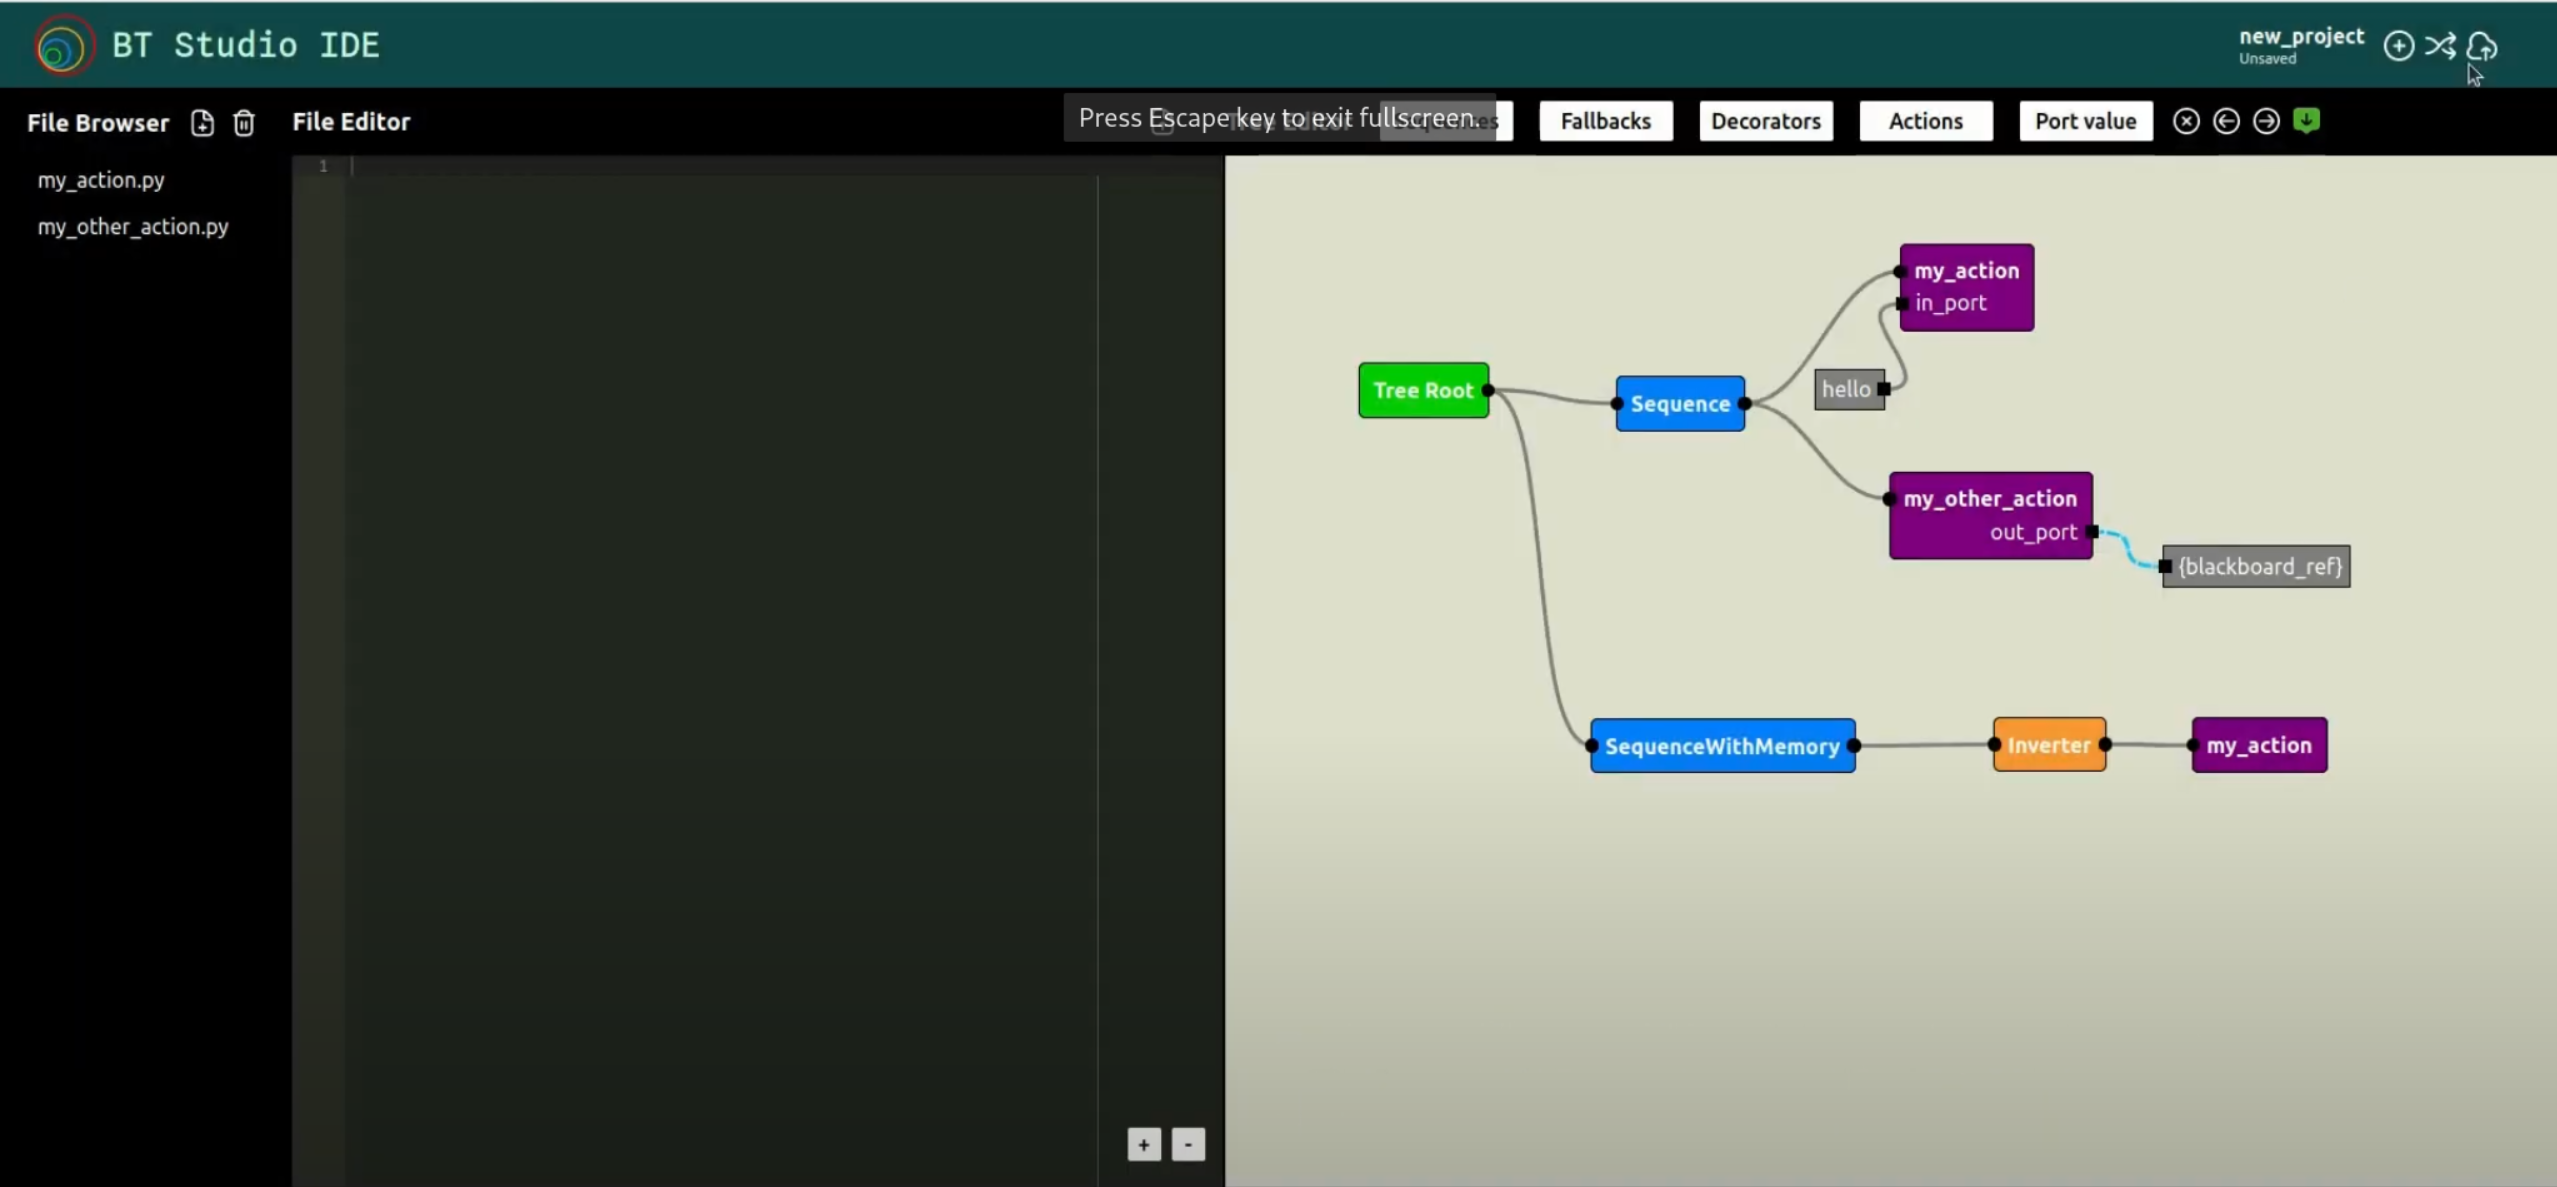
\includegraphics[width=0.8\textwidth]{figures/bt-studio/bt-old.png}
    \caption{Apariencia antigua de BT Studio}
    \label{fig:bt-old-ref}
\end{figure}

Con todo esto, lo que más interesa para las mejoras son los siguientes apartados:

% \subsection{Estructura de la plataforma}

% El objetivo de BT Studio es proporcionar una interfaz web versátil y de fácil uso que permita a los usuarios la creación de aplicaciones robóticas complejas usando árboles de comportamiento. Para esto es necesario establecer las distintas funcionalidades que serán la base de la plataforma:

% \begin{itemize}
%     \item Un IDE web que sirva como interfaz única para el usuario. Desde este, el usuario debe ser capaz de crear diferentes aplicaciones robóticas, guardarlas, editarlas y ejecutarlas. 
%     \item Se debe realizar la traducción desde los ficheros que conforman una aplicación en BT Studio a código ejecutable. Esto debe ocurrir de forma totalmente transparente para el usuario, es decir, que el usuario debe poder ejecutar la aplicación robótica creada en el web IDE sin necesitar configurar nada.
%     \begin{figure}[H]
%         \centering
%         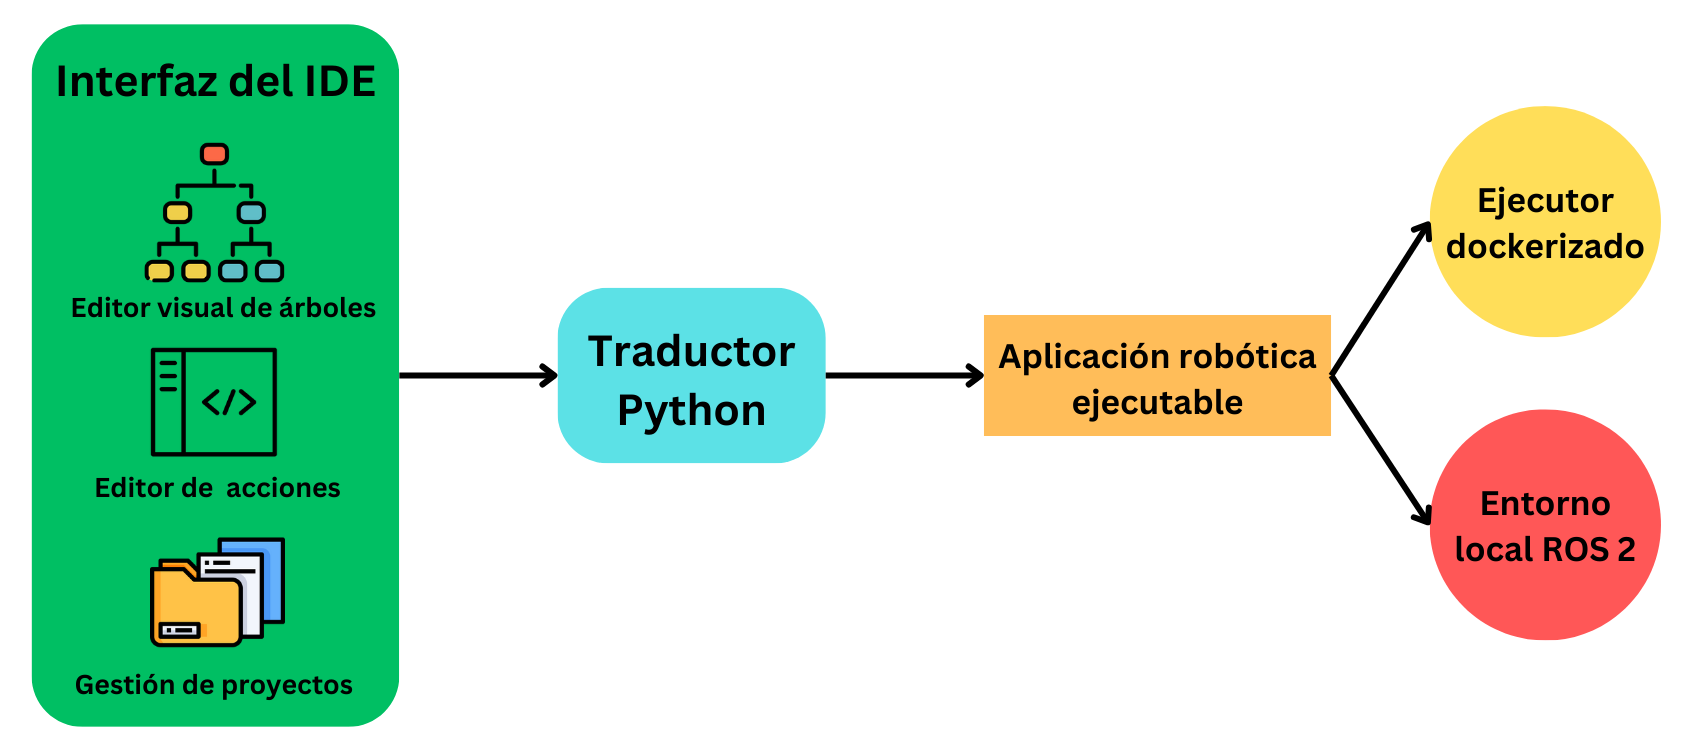
\includegraphics[width=0.9\textwidth]{figures/bt-studio/app_pipeline.png}
%         \caption{Proceso de generación antiguo de aplicaciones en BT Studio}
%         \label{fig:ejemplo}
%     \end{figure}
%     \item Se debe dotar al usuario en el web IDE de herramientas en el web IDE para la visualización y depuración de la ejecución de la aplicación robótica. Esto requiere de al menos proporcionar una interfaz para iniciar, pausar y reiniciar la ejecución que se realice dentro del entorno de ejecución de BT Studio, es decir, en el Robotics Backend, cuyo funcionamiento se explico en el capitulo \ref{cap:tecnologias}.
% \end{itemize}

% Para la comunicación con el RAM (Robotics Application Manager) , el RADI define un protocolo de comunicación a través de WebSockets. BT Studio implementa este protocolo para realizar acciones en el entorno de ejecución desde la interfaz del IDE. 

% \begin{figure}[H]
%     \centering
%     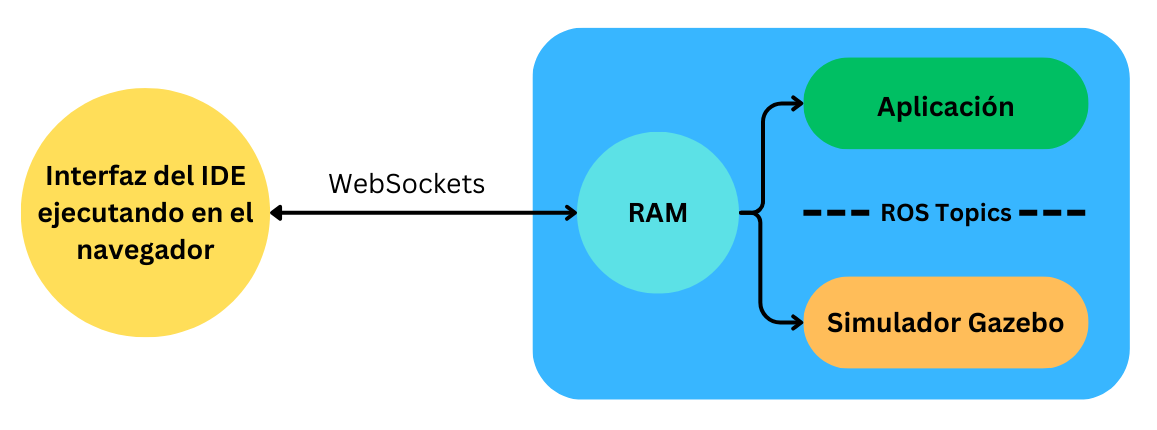
\includegraphics[width=0.9\textwidth]{figures/bt-studio/docker_exec_v2.png}
%     \caption{Ejecución de una aplicación robótica en un entorno dockerizado}
%     \label{fig:ejemplo}
% \end{figure}

\subsection{Definición de aplicaciones robóticas en BT Studio}

En BT Studio, una aplicación robótica basada en árboles de comportamiento está definida por dos componentes: 

\begin{itemize}
    \item \textbf{Acciones:} programada cada una en un fichero Python, siguiendo la estructura estándar para la definición de acciones que proporciona la librería PyTrees. Estas se editan mediante el editor de texto incluido en BT Studio. Cada acción es una clase que implementa distintos métodos propios de un nodo de ejecución de un árbol de comportamiento, como \textit{initialise}, \textit{update} (equivalente a \textit{tick} en PyTrees) o \textit{terminate}. 
    \lstinputlisting[
        float,
        floatplacement=!htp,
        language=Python,
        label=cod:base\_action,
        caption=Estructura de una acción en BT Studio
    ]{code/base_action.py}

    \item \textbf{Árbol de comportamiento:} definidos de manera gráfica mediante el editor visual de BT Studio, que permite definir gráficos personalizados con toda la semántica necesaria para definir un árbol de comportamiento. Estos son guardados en formato JSON. Los nodos de control de flujo disponibles son aquellos definidos por la librería BT.cpp. 
    \begin{figure}[H]
        \centering
        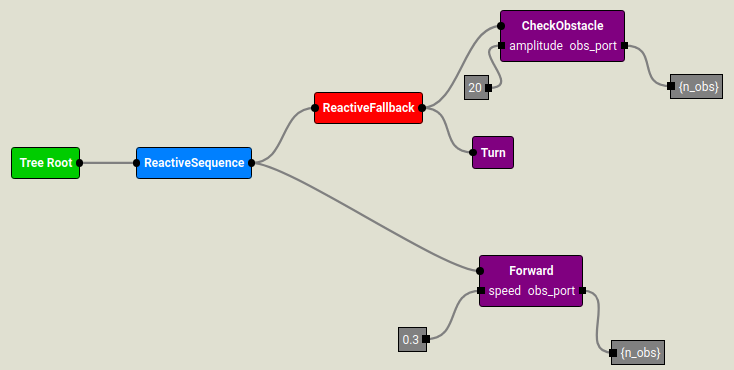
\includegraphics[width=0.7\textwidth]{figures/bt-studio/tree_example.png}
        \caption{Árbol de comportamiento antiguo creado con BT Studio}
        \label{fig:ejemplo}
    \end{figure}
    
\end{itemize}

Todas las aplicaciones que los usuarios crean, editan y ejecutan están basadas en estas funcionalidades básicas. Todos los archivos asociados a una aplicación concreta constituyen un proyecto robótico. 

\subsection{Estructura de un proyecto}\label{sec:bt-struct-old}

La estructura de un proyecto está dividida en dos secciones, el directorio \textit{actions} donde están las acciones y el fichero \textit{graph.json} que guarda el árbol de comportamiento. 

\begin{figure}[H]
    \centering
    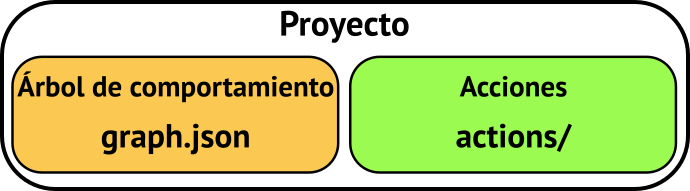
\includegraphics[width=0.7\textwidth]{figures/bt-studio/bt-proy-old.png}
    \caption{Estructura antigua de un proyecto de BT Studio}
    \label{fig:estructura-antigua}
\end{figure}


\subsection{Gestor de comunicaciones: CommsManager}

Este componente se encarga de la comunicación entre el frontend de BT Studio y el entorno de ejecución dockerizada. Implementa distintas funciones para la comunicación mediante mensajes Websocket con un formato determinado. El protocolo concreto para esa comunicación está definido posteriormente en la sección \ref{sec:conex}. 

Este gestor está definido como un \textit{singleton}, es decir, solo se puede crear una instancia, que se pasa a los distintos componentes para que puedan interactuar con el entorno dockerizado. Al ser único, toda la comunicación de este tipo está centralizada para todo BT Studio

\begin{figure}[H]
    \centering
    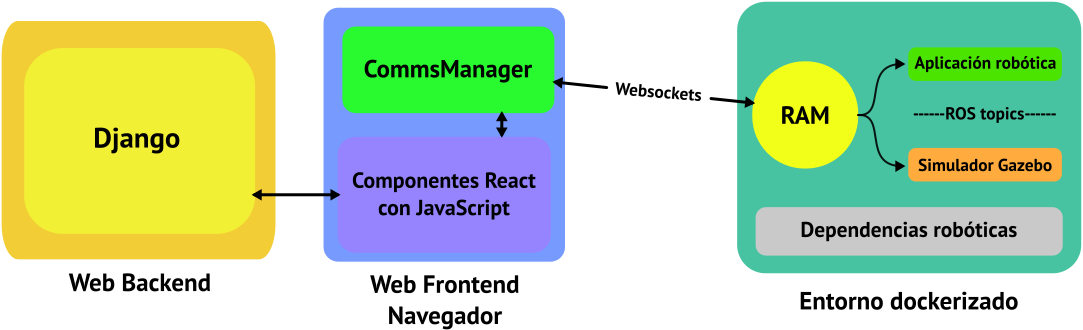
\includegraphics[width=\textwidth]{figures/bt-studio/bt-structure-old.png}
    \caption{Diseño antiguo de la estructura de BT Studio}
    \label{fig:bt-old-old-ref}
\end{figure}